% Unified paper: synthesizes Notes 01-03 and motivates multi-week (weekly-unit) forecasting.
% Compile: pdflatex paper_multiweek_forecasting.tex (run twice for refs).
% Figures in ./figures/ (fig1, fig11, fig12, fig13, fig14).
\documentclass[11pt]{article}
\usepackage[margin=1in]{geometry}
\usepackage{amsmath,amssymb}
\usepackage{graphicx}
\usepackage{booktabs}
\usepackage{float}
\usepackage{xcolor}
\usepackage[colorlinks=true,linkcolor=blue,citecolor=blue,urlcolor=blue]{hyperref}
\graphicspath{{figures/}}

\newcommand{\veh}{\,\text{veh/h}}
\title{\textbf{The Week Is the Unit}\\[3pt]
\large Multi-Week Highway Traffic Forecasting as Level Dynamics}
\author{Traffic Forecasting Project}
\date{June 2026}

\begin{document}
\maketitle

\begin{abstract}
\sloppy
\noindent
We study one-week-ahead and multi-week-ahead forecasting of California highway
traffic \emph{flow}, using five years of Caltrans loop-detector data (the LargeST
Greater Bay Area subset; 2{,}352 sensors, 2017--2021, hourly). Two results frame
the paper. First, the \emph{one-week} problem is, for practical purposes,
\textbf{solved by a simple, interpretable model}: a recency-weighted seasonal
baseline plus an explicit holiday adjustment reaches $R^2=0.949$ and a
weekly-aggregate MAPE of $3.55\%$, and we show -- by bounding autoregressive
modeling, learned calendar/sensor features (ridge/XGBoost), and an oracle noise
floor -- that essentially no further skill is recoverable at the hourly
granularity. Traffic at short horizons is ``sunrise-like'': dominated by a
deterministic cycle anchored to human schedules. Second, and our main thesis, the
\emph{interesting} problem begins at \textbf{multi-week horizons}, and it should
be posed in the natural temporal unit of \textbf{weeks, not hours}. We decompose
flow into a frozen hourly \emph{shape}, an averaging \emph{noise} term, and a
slowly varying \emph{level}; the first two are solved or irreducible, so all
multi-week forecasting signal lives in the per-sensor weekly \emph{level} series.
That series is a short ($\sim$52 points/year), classic macro time series --
$94\%$ annual-seasonal with an autocorrelated remainder pre-COVID -- on which
trend models, exogenous macro covariates, and state-space methods apply. We
characterize when multi-week forecasting becomes worthwhile (a smooth onramp from
$\approx$3--4 weeks), reframe it as weekly-level forecasting, and lay out the
model families suited to it. Testing a ladder of those models -- rules, fitted
classical, pooled-panel, and trained global ML -- we find that on \emph{endogenous}
information the simplest recency rule sits at the ceiling and training does not beat
it, the same lesson as one week. This verdict is conditional on a limited sample,
and we test its leading escape route -- pooling more regions -- directly: a strong
statewide common level factor exists but is contemporaneous and \emph{unforecastable}
(white in time), so cross-regional pooling aids nowcasting, not multi-week
forecasting. More years and known-ahead covariates remain the open levers.
\end{abstract}

\section{Introduction}
Short-term traffic forecasting (5--60 minutes) is a mature field dominated by
spatio-temporal deep models. Much less attention has gone to the
\emph{week-to-several-weeks} horizon that matters for operations and planning:
staffing, maintenance scheduling, demand management, and infrastructure analysis.
This paper makes two points about that regime.

The first is deflationary. We show that forecasting hourly flow \emph{one week}
ahead is essentially solved by a trivial seasonal rule plus a holiday correction,
and that the usual escalation -- autoregressive residual models, gradient-boosted
feature models -- buys nothing, because it is modeling structure that the seasonal
baseline has already removed or that is irreducible noise. The constructive payoff
is knowing exactly \emph{why} and \emph{where} the easy regime ends.

The second is programmatic. As the horizon grows, the deterministic weekly cycle
that makes short-horizon forecasting easy contributes the same (zero) error, while
a slowly drifting \emph{level} -- coupled to the annual cycle and, ultimately, the
macroeconomy -- comes to dominate forecast uncertainty. We argue this regime is a
problem in its own right, with a different natural unit (the week), a different
signal (level dynamics), different models (trend / state-space / covariate-driven),
and different value (planning). We give the empirical case and a concrete modeling
agenda, including recommendations for tasks like ``total road traffic 4--6 weeks
out.''

\paragraph{Contributions.}
(1) A synthesis showing one-week hourly flow forecasting is at its practical
ceiling, with the negative results that establish it
(\S\ref{sec:oneweek}). (2) A level/shape/noise decomposition explaining why
(\S\ref{sec:decomp}). (3) A characterization of the multi-week onramp and the
horizon at which richer modeling pays (\S\ref{sec:onramp}). (4) The reframing of
multi-week forecasting as weekly-\emph{level} forecasting, with an empirical
decomposition of that series (\S\ref{sec:weekly}). (5) A model taxonomy and
recommendations for the weekly, multi-week problem (\S\ref{sec:models}).

\section{Related work}
\label{sec:related}
\paragraph{Short-horizon spatio-temporal traffic forecasting.} The dominant
paradigm forecasts traffic minutes-to-hours ahead by modeling spatial dependence
across sensors. Seeded by the METR-LA and PEMS-BAY benchmarks (Li et al., 2018), it
produced a long line of spatio-temporal graph networks: DCRNN (Li et al., 2018),
STGCN (Yu et al., 2018), Graph WaveNet (Wu et al., 2019), ASTGCN (Guo et al., 2019),
AGCRN (Bai et al., 2020), and more recent DSTAGNN, DGCRN, and D2STGNN. LargeST (Liu
et al., NeurIPS 2023), the dataset we use, was built to scale this line to thousands
of sensors and benchmarks twelve such models at the standard $\sim$3-hour (12-step)
horizon. Tellingly, its framing is the inverse of ours: the headline result is that
purely temporal baselines -- ``Historical Last'' (a seasonal-naive) and LSTM --
perform \emph{worst}, precisely because they ignore spatial correlation. The field
is organized around spatial modeling at short horizons.

\paragraph{Long-horizon time-series forecasting.} A parallel literature forecasts
hundreds of steps ahead on a fixed ``Traffic'' occupancy benchmark via transformers
-- Informer (Zhou et al., 2021), Autoformer (Wu et al., 2021), PatchTST (Nie et al.,
2023) -- and decomposition networks such as N-HiTS and TimesNet. Notably, Zeng et
al.\ (2023) showed that a single linear layer (DLinear) rivals or beats these
transformers -- a direct precedent for our finding that a one-parameter rule beats
pooled ARIMA and gradient boosting. But ``long-term'' here still means hourly steps
over hours to a day or two (e.g.\ LSTTN, 2024); recent time-series foundation models
(Chronos, TimesFM, Moirai, 2024) extend horizons by pretraining on large corpora but
are not specialized to this reframing.

\paragraph{The gap.} Across both strands we find no work that (i) forecasts traffic
at multi-week horizons, (ii) adopts the \emph{week} as the modeling unit, or (iii)
treats the slowly-varying \emph{level}/trend as the forecasting object. Classical
structural and seasonal methods -- ETS/Holt--Winters, (S)ARIMA, STL (Cleveland et
al., 1990), Bayesian structural time series (Scott and Varian, 2014) -- are the
natural tools for that object yet are essentially unused on these datasets. Our
reframing occupies this gap and yields a clean contrast on a \emph{single} dataset:
spatial graph networks beat simple temporal baselines at three hours, while at
multiple weeks the reverse holds -- recency rules beat pooled and learned models and
spatial structure stops helping. The seasonal-naive that the spatio-temporal
literature reports as its weakest baseline is, at multi-week horizons, near the
ceiling.

\section{Data and setup}
\label{sec:data}
We use \textbf{LargeST} (Liu et al., NeurIPS 2023), assembled from the Caltrans
Performance Measurement System (PeMS): inductive-loop detectors reporting
\emph{flow} (vehicles/hour), occupancy, and speed. We take the \textbf{Greater Bay
Area} subset (Caltrans District 4, $N=2{,}352$ mainline sensors), 2017--2021,
aggregate the 5-minute series to hourly, and forecast flow -- the most seasonal of
the three channels (the same baseline on a speed dataset, PEMS-BAY, reaches only
$R^2\approx0.76$: speed is dominated by irreducible congestion noise and is a
genuinely harder target). The data form a matrix $Y\in\mathbb{R}^{T\times N}$,
$y_{i,t}$ the mean flow at sensor $i$ in hour $t$; missing values ($\sim$2\%) are
imputed per sensor by hour-of-week mean. The weekly period is $P=24\times7=168$
hours and $\phi(t)=t\bmod P$ is the hour-of-week. Unless noted, models are trained
on 2017--2018 and tested on 2019 in a rolling-origin backtest; the pre-pandemic
years isolate steady-state behaviour, with 2020--2021 reserved to illustrate
regime change.

\section{The one-week problem is solved}
\label{sec:oneweek}

\paragraph{A seasonal baseline.} Because flow is dominated by a weekly commute
cycle (Figure~\ref{fig:profile}), a natural predictor of any cell is its recent
average at the same hour-of-week,
$b_{i,t}=\tfrac14\sum_{k=1}^{4} y_{i,t-Pk}$. Every lag is a multiple of a week, so
$b$ is computable for the entire week ahead with no leakage. It explains
$\mathbf{93.6\%}$ of hourly variance out-of-sample (per-sensor median $R^2=0.91$).

\begin{figure}[H]\centering
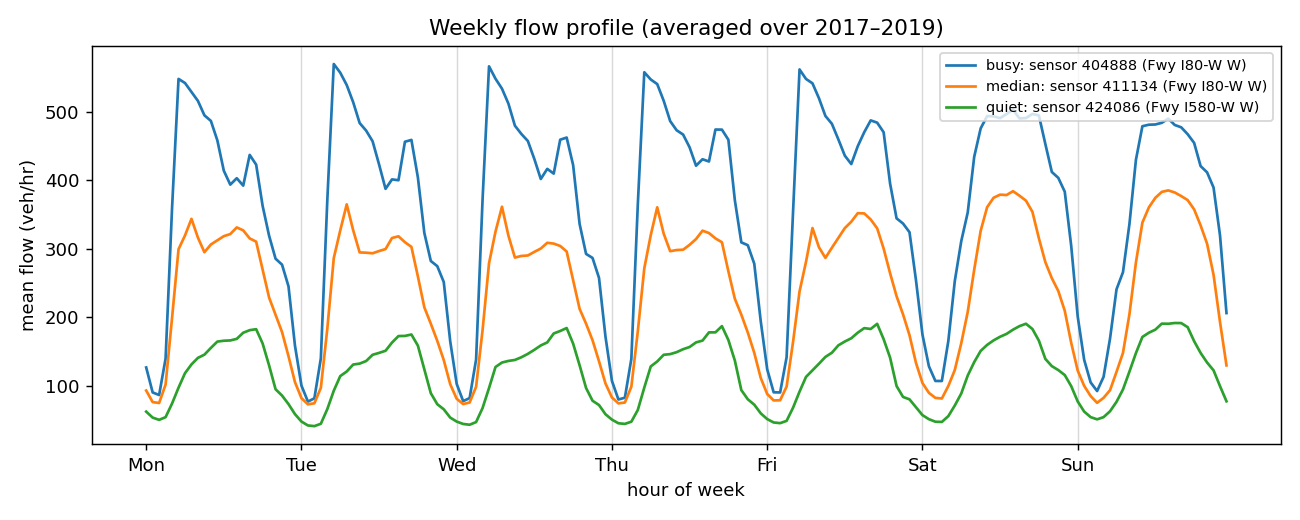
\includegraphics[width=0.95\linewidth]{fig1_weekly_profile.png}
\caption{Mean flow by hour-of-week for three sensors. The weekday commute
double-peak and weekend single-hump repeat with high regularity -- the
deterministic ``shape'' that makes short-horizon forecasting easy.}
\label{fig:profile}
\end{figure}

\paragraph{Recency and holidays.} Two interpretable refinements push past the
baseline. (i) Replacing the flat 4-week mean with an \emph{EWMA} over weekly lags
($w_k\propto\alpha^{k-1}$, $\alpha\approx0.8$) lifts $R^2$ to $0.9435$; free weekly
weights do no better. (ii) An explicit \emph{holiday model} -- a pooled
per-(holiday-identity, hour-of-day) multiplicative factor on the baseline --
targets the fact that holidays are $8\%$ of hours but $\sim$23\% of squared error;
it cuts holiday-window RMSE from $67$ to $48\veh$ and \emph{stacks} with EWMA.
Combined: $\mathbf{R^2=0.9493}$, weekly-aggregate MAPE $\mathbf{3.55\%}$
(Table~\ref{tab:prog}).

\begin{table}[H]\centering
\caption{Rolling-origin one-week-ahead backtest, 2019 (359 origins $\times H{=}168$).}
\label{tab:prog}
\begin{tabular}{lcccc}
\toprule
Model & $R^2$ & RMSE all & RMSE ordinary & RMSE holiday \\
\midrule
Flat seasonal baseline   & 0.9404 & 40.14 & 37.06 & 66.96 \\
EWMA $\alpha{=}0.8$      & 0.9435 & 39.10 & 35.98 & 65.99 \\
EWMA $+$ holiday         & \textbf{0.9493} & \textbf{37.01} & 35.98 & 47.71 \\
\bottomrule
\end{tabular}
\end{table}

\paragraph{The escalation does not help.} Modeling the residual
$r=y-b$ with its own dynamics or with learned features yields almost nothing.
Autoregression: recent-lag predictability is strong at $h{=}1$ ($R^2{=}0.63$) but
collapses by a week out, for an aggregate-$R^2$ ceiling of $+0.0027$; a cleaner
weekly-aggregate AR caps at $+0.0010$. Learned features (the natural ridge/XGBoost
setup) are bounded by their group means out-of-sample (Table~\ref{tab:feat}):
hour-of-week / day-of-week / hour-of-day explain $\approx0$ \emph{by construction}
(the baseline already is the hour-of-week mean); only week-of-year carries a tiny,
holiday-redundant signal; high-cardinality interactions overfit. ML cannot
manufacture signal the construction removed.

\begin{table}[H]\centering
\caption{Out-of-sample residual variance explained by each feature's group means
(an upper bound for any ridge/XGBoost model on that feature).}
\label{tab:feat}
\begin{tabular}{lcc}
\toprule
Feature on the residual & OOS residual $R^2$ & Aggregate $R^2$ lift \\
\midrule
hour-of-week / day-of-week / hour-of-day & $\le 0$ & $0$ \\
week-of-year (52)            & $+0.008$ & $+0.0005$ \\
week-of-year $\times$ lanes  & $+0.009$ & $+0.0005$ \\
week-of-year $\times$ sensor & $-0.045$ & (overfits) \\
\bottomrule
\end{tabular}
\end{table}

\paragraph{We are at the floor.} Fitting \emph{oracle} structure in-sample on 2019
(perfect parameters, an upper bound) gives $R^2=0.938$ for a static weekly-seasonal
mean and $0.943$ with an oracle holiday effect -- both \emph{below} our
out-of-sample $0.949$, because the EWMA tracks within-year nonstationarity a static
mean cannot. With every endogenous lever bounded near zero, the remaining
$\sim$5\% is dominated by irreducible idiosyncratic noise (incidents, weather,
one-offs). One-week hourly flow forecasting is solved.

\section{Why: a level / shape / noise decomposition}
\label{sec:decomp}
Write flow as a slowly varying level times a normalized weekly shape, plus noise:
\begin{equation}
y_{i,t} \;=\; \underbrace{L_{i,w(t)}}_{\text{weekly level}}\;\cdot\;
\underbrace{S_{i,\phi(t)}}_{\text{hourly shape}}\;+\;\underbrace{\varepsilon_{i,t}}_{\text{noise}},
\label{eq:decomp}
\end{equation}
where $w(t)$ is the week index. The three terms behave completely differently with
forecast lead $h$:
\begin{itemize}
\item \textbf{Shape} $S$ is anchored to the clock and calendar (hence to the sun):
  deterministic given the date, contributing \emph{zero} error at \emph{any} $h$.
  Empirically it is frozen -- the normalized weekly profile has cross-year
  correlation $\ge0.99$ across 2017--2021 (Figure~\ref{fig:stab}).
\item \textbf{Noise} $\varepsilon$ is irreducible but bounded and \emph{averages
  down} under aggregation -- the reason the weekly-aggregate MAPE is only $3.5\%$.
\item \textbf{Level} $L$ is a near-random walk: its forecast variance \emph{grows}
  with $h$. At one week it is negligible against $S$; at months it is everything.
\end{itemize}
This explains \S\ref{sec:oneweek}: one-week models work on $S$ (solved) and
$\varepsilon$ (irreducible), so there is nothing left. It also predicts where the
problem gets hard -- as $h$ grows and $L$'s contribution rises -- and contrasts
traffic with asset prices, which are almost \emph{all} level band (no seasonal
anchor) and whose structure is arbitraged away, hard even at $h{=}1$. Traffic's
seasonal anchor is not arbitraged away, so it is easy short-term and only becomes
price-like as the horizon erodes the anchor's weight.

\begin{figure}[H]\centering
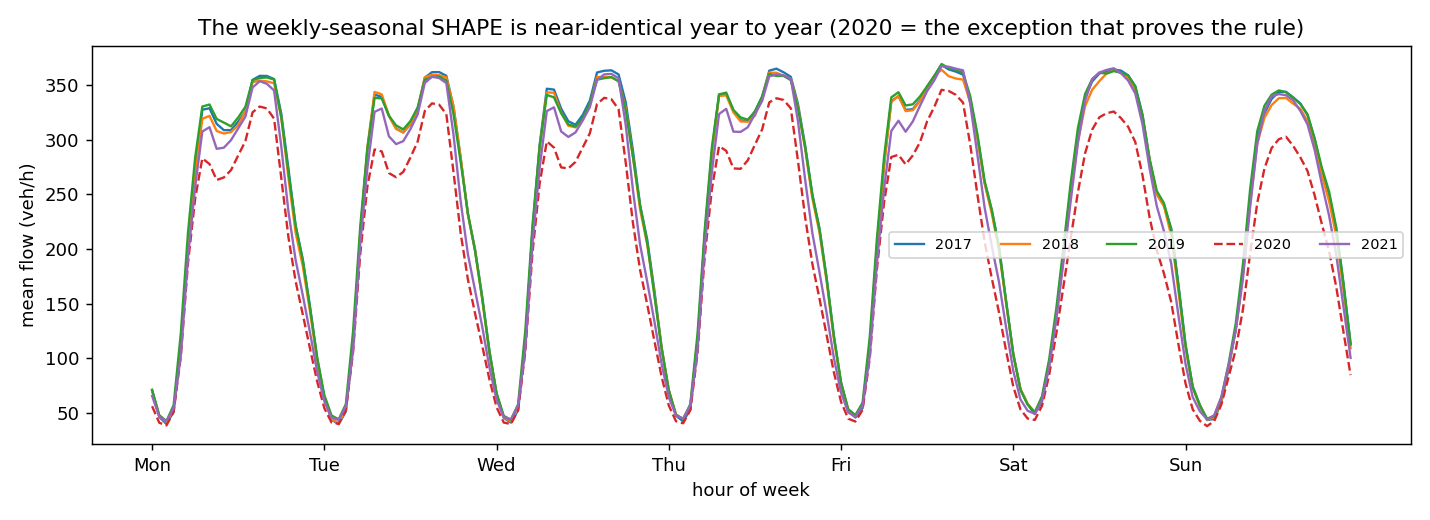
\includegraphics[width=0.95\linewidth]{fig12_seasonal_stability.png}
\caption{The weekly-seasonal \emph{shape} $S$ is near-identical year to year
($\ge0.99$ correlation); 2020 (dashed) drops the \emph{level} and flattens the
commute peaks under remote work but preserves the shape.}
\label{fig:stab}
\end{figure}

\section{The multi-week onramp}
\label{sec:onramp}
A leakage constraint governs multi-week horizons. To forecast target week $w$, the
origin sits $H$ weeks earlier, so the weekly lag at distance $k$ (the week $w{-}k$)
is observable only if $w{-}k$ lies at or before the origin, i.e.\ $k\ge H$. The
one-week baseline ($H{=}1$) therefore averages the four most recent weeks
$\{1,2,3,4\}$; at $H$ weeks ahead the four \emph{most recent observable} weeks are
$\{H,H{+}1,H{+}2,H{+}3\}$ -- e.g.\ $\{4,5,6,7\}$ at four weeks and $\{8,9,10,11\}$ at
eight. The seasonal \emph{shape} is still captured, but the \emph{level} estimate is
drawn from increasingly stale data (two months old at $H{=}8$, possibly across a
sub-annual seasonal boundary). We isolate this with a
horizon-\emph{independent} floor -- a \emph{centered oracle} averaging weeks
$\{\pm1,\pm2\}$ around the target (it peeks at the future, so has perfect
concurrent level: RMSE $38.1\veh$ at every $H$). The gap between the naive baseline
and this floor is the prize a better level model could win
(Figure~\ref{fig:sweep}, Table~\ref{tab:sweep}).

\begin{figure}[H]\centering
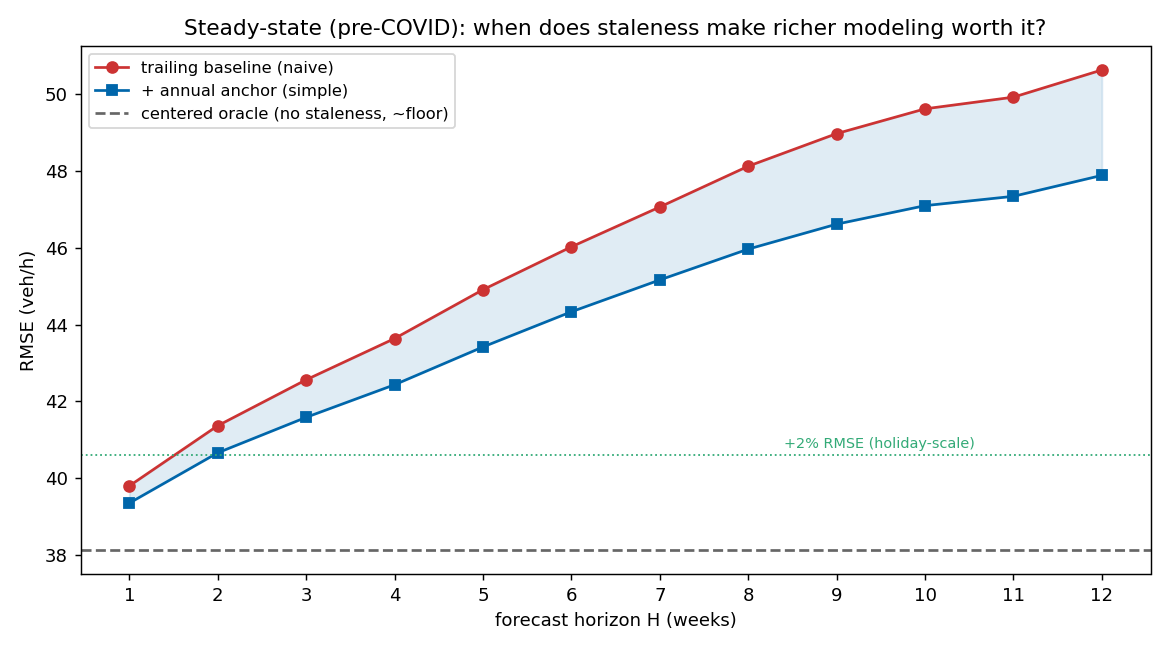
\includegraphics[width=0.86\linewidth]{fig13_horizon_sweep.png}
\caption{Steady-state RMSE vs.\ horizon (pre-COVID, test 2019). The naive baseline
pulls away from the no-staleness floor roughly linearly; the shaded band is the
recoverable prize. A simple annual anchor recovers about half; the rest needs
genuine trend modeling. ``Interesting'' begins at $H\approx3$--$4$ weeks.}
\label{fig:sweep}
\end{figure}

\begin{table}[H]\centering
\caption{Steady-state horizon sweep. Gap-to-floor is the share of RMSE due to
level staleness -- the target for richer modeling.}
\label{tab:sweep}
\begin{tabular}{cccc}
\toprule
Horizon & Naive RMSE & Gap to floor & Optimal annual weight \\
\midrule
1 week & 39.8 & \phantom{0}4\% & 0.20 \\
2 weeks & 41.4 & \phantom{0}8\% & 0.23 \\
4 weeks & 43.6 & 13\% & 0.27 \\
8 weeks & 48.1 & 21\% & 0.34 \\
12 weeks & 50.6 & 25\% & 0.39 \\
\bottomrule
\end{tabular}
\end{table}

There is \textbf{no sharp knee}: each week of horizon ages the anchor by a week and
adds roughly constant level-drift variance, so the gap grows $\sim$linearly,
$4\%\to13\%\to25\%$ over 1--12 weeks. Below $\sim$2 weeks the naive rule is within
noise of the floor; at $\mathbf{H\approx3\text{--}4}$ weeks the recoverable gap
reaches the scale of gains already worth building (the holiday model's $\sim$2\%
RMSE); by 8--12 weeks a quarter of the error is level staleness. The recoverable
signal is, by construction, in the \emph{level}.

\section{Reframing: multi-week forecasting is weekly-\emph{level} forecasting}
\label{sec:weekly}
The decomposition \eqref{eq:decomp} and the onramp point to a single reframing.
Since $S$ is frozen and known, the $H$-week-ahead forecast factorizes:
\begin{equation}
\hat y_{i,t+H\cdot P}\;=\;\hat L_{i,\,w+H}\;\cdot\;S_{i,\phi}\quad(\text{plus the holiday factor}),
\end{equation}
so \textbf{all multi-week difficulty collapses onto forecasting the per-sensor
weekly level series} $L_{i,w}=\text{mean}_{t\in w}\,y_{i,t}$. This is the right
object, and the right \emph{unit}: weeks, not hours. Per sensor over 2017--2019 the
hourly series has $26{,}208$ points dominated by the deterministic daily/weekly
cycle, whereas the weekly-level series has just $156$ points ($\sim$52/year) and
looks like an ordinary macro time series (Figure~\ref{fig:level}).

\begin{figure}[H]\centering
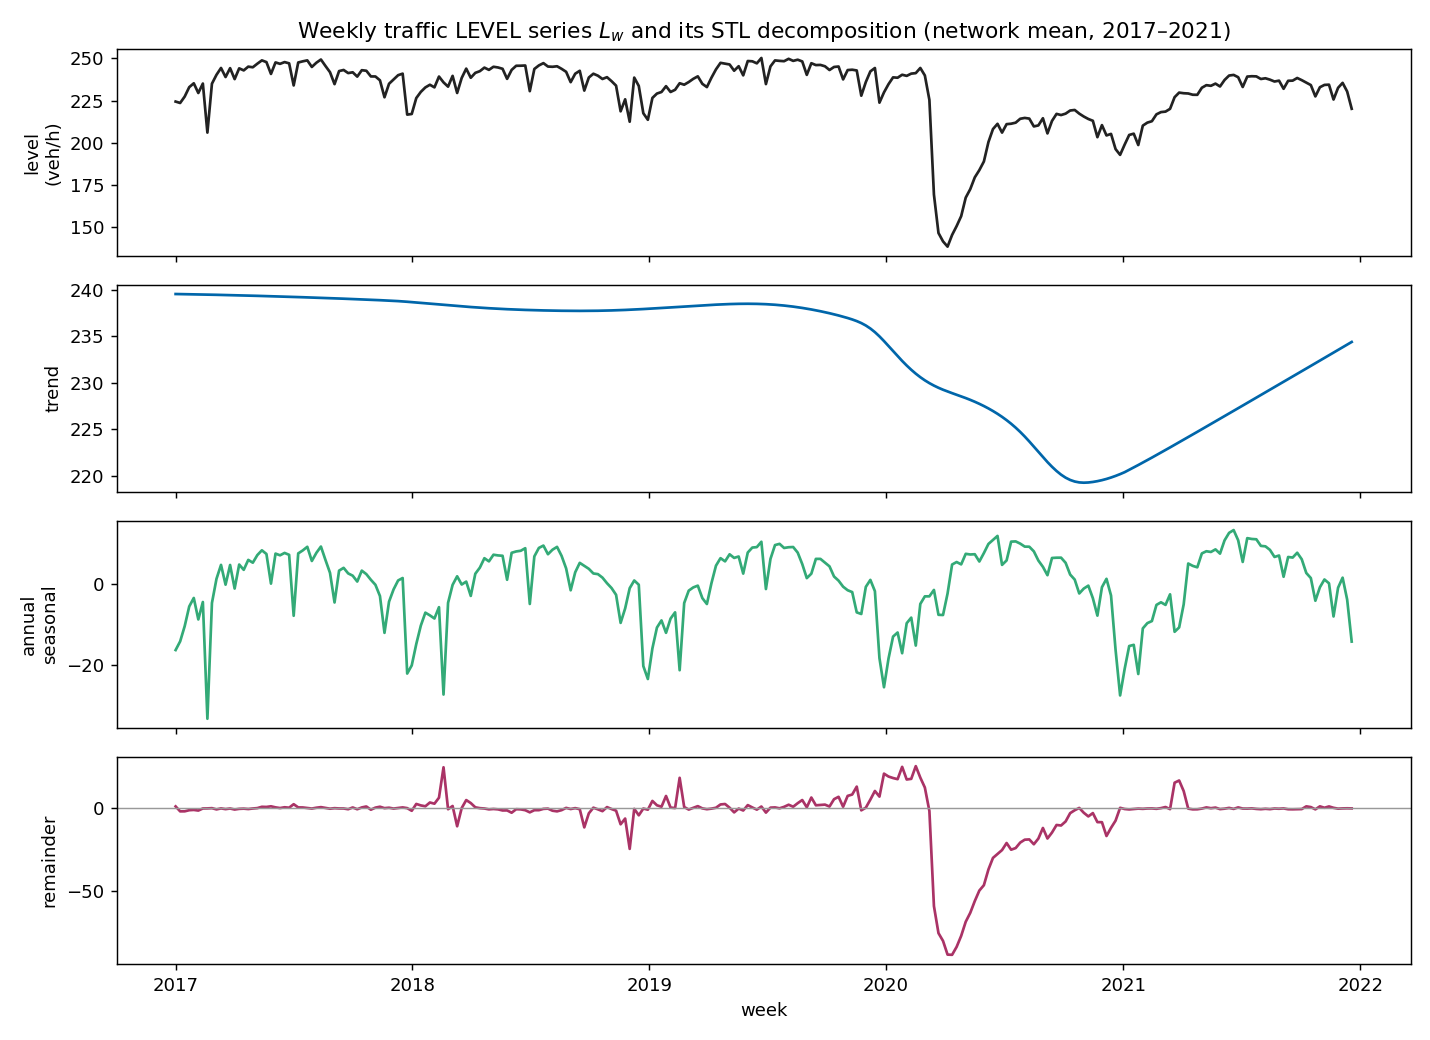
\includegraphics[width=0.95\linewidth]{fig14_weekly_level.png}
\caption{The weekly traffic level $L_w$ (network mean) and its STL decomposition.
Pre-COVID, the series is $94\%$ annual-seasonal, $1.4\%$ trend, $4.2\%$ remainder,
and the remainder is autocorrelated (lag-1 $0.30$, lag-3 $0.40$) -- a short,
forecastable macro series. The 2020 break appears as a trend/remainder excursion.}
\label{fig:level}
\end{figure}

Empirically the weekly level is exactly the kind of series classical forecasting
was built for: a dominant smooth \emph{annual} cycle, a slow trend, and a
modestly autocorrelated remainder. Crucially, the annual cycle that dominates
$L_w$ is precisely the sub-annual seasonal variation the hourly trailing baseline
\emph{misses} at long horizons (it goes stale across the year) -- which is why the
``annual anchor'' recovered part of the onramp gap in \S\ref{sec:onramp}. Posing
the problem in weeks unifies these observations and decouples the easy part (the
frozen hourly shape) from the hard part (level dynamics).

\section{Models for weekly, multi-week forecasting}
\label{sec:models}
Reframed as forecasting $L_{i,w}$ several weeks ahead (e.g.\ ``total road traffic
4--6 weeks out''), the problem becomes a short, seasonal, covariate-driven time
series -- a different model class than short-term spatio-temporal nets. We
recommend, roughly in increasing ambition:

\begin{enumerate}
\item \textbf{Classical univariate baselines.} Holt--Winters / ETS and
  \textbf{(S)ARIMA with annual season $s{=}52$}, or \textbf{STL + ARIMA} on the
  remainder. These directly capture trend $+$ annual seasonal $+$ AR remainder and
  are strong, hard-to-beat baselines on a 52-point-per-year series. For
  ``total traffic 4--6 weeks out'' on a single corridor or the network aggregate,
  an STL/ETS model is the natural first choice.
\item \textbf{Structural / state-space models.} Unobserved-components and Bayesian
  structural time series (BSTS), dynamic linear models. They model
  level $+$ trend $+$ seasonal explicitly, yield \emph{calibrated uncertainty}
  (which grows with horizon -- essential for planning), and accommodate
  \emph{level shifts}, giving graceful behaviour around regime changes.
\item \textbf{Dynamic regression with exogenous covariates} (ARIMAX /
  regression-with-ARMA-errors). This is where the real multi-week headroom is, and
  the decisive constraint is \emph{availability at inference time}: a covariate
  helps a $6$-week forecast only if its future value is known then. \emph{Known
  exactly ahead} -- school/academic calendar, public-holiday density, scheduled
  large events (sport/concerts), and planned lane closures / roadwork -- is ideal,
  and a natural generalization of the holiday model (a known-ahead calendar anomaly
  the seasonal baseline misses). \emph{Slowly varying, observable at the origin} --
  fuel prices (or their futures curve), employment / mobility indices -- is usable
  via persistence. \emph{Needs its own forecast} -- weather -- is weaker, since
  precipitation skill decays over the horizon. Bringing the known-ahead signals in
  is the single most promising direction, because it adds information the
  endogenous series lacks (cf.\ \S\ref{sec:oneweek},\,\S\ref{sec:ladder}:
  complexity must follow information, not precede it). A caveat on granularity:
  short, localized events wash out of the weekly-network aggregate and pay off only
  at the sensor/corridor level near the venue or closure.
\item \textbf{Hierarchical / global panel models.} The object is a
  $156\text{-week}\times2352\text{-sensor}$ panel with strong shared structure
  (corridors, region, sensor type). A single \emph{global} model -- hierarchical
  Bayesian, or gradient-boosted / global neural forecasters (LightGBM on lag$+$
  calendar$+$covariate features, DeepAR, Temporal Fusion Transformer) trained
  across all sensors with sensor embeddings -- pools strength across the short
  per-sensor series and tends to dominate purely-local fits. Reconciliation across
  the sensor hierarchy (corridor $\to$ region totals) is natural here.
\item \textbf{Gaussian processes} with a smooth trend kernel plus a periodic
  (annual) kernel, for flexible probabilistic interpolation/extrapolation of the
  level on short series.
\item \textbf{Regime-aware models.} Markov-switching or online change-point methods
  for robustness to structural breaks (the COVID failure mode), valuable when the
  cost of large transient errors is high.
\end{enumerate}

\paragraph{A concrete recommendation.} For ``total traffic on a road 4--6 weeks
out'': model the weekly aggregate as a \textbf{dynamic-regression / structural
time-series} with an annual seasonal component and a handful of known-ahead
covariates (academic calendar, holiday density, medium-range weather), and report
a predictive \emph{distribution}, not a point. Where many sensors/roads are
forecast jointly, fit a \textbf{global gradient-boosted or DeepAR-style model on
the weekly panel} with sensor embeddings and the same covariates, reconciled up the
spatial hierarchy. The short series length ($\sim$52/year) favours structured or
globally-pooled models over data-hungry local deep nets.

\section{Empirical: do trained models beat rules on the weekly level?}
\label{sec:ladder}
We tested the ladder directly -- parameter-free rules, a fitted classical model, a
pooled (panel) model, and a trained global ML model -- forecasting $L_{i,w}$ four
weeks ahead on the full 2{,}352-sensor panel (train 2017--18, test 2019;
Table~\ref{tab:ladder}). The result mirrors the one-week finding: the simplest
recency rule is at the ceiling, and training does not beat it. A trailing mean of
the four most recent observable weeks reaches $R^2=0.961$; the only thing that
improves on it is a \textbf{one-parameter} convex blend toward the prior-year
value ($0.9626$). A pooled direct AR with coefficients shared across all sensors
\emph{under}performs the rule, even after replacing the noisy 52 week-of-year means
with a smooth low-variance \emph{Fourier} seasonal (which helped the pooled model,
$0.9465\!\to\!0.9501$, but not enough); a trained gradient-boosted global model is
worse still, overfitting the short history. On a series that is already $96\%$
predictable from recency, ``near-optimal estimate $+$ tiny shrinkage'' beats every
attempt to reconstruct the level from components.

\begin{table}[H]\centering
\caption{Weekly-level forecasting at $H{=}4$ weeks, test 2019, all 2{,}352 sensors.
$R^2$ here is flattered (see below); RMSE is the honest comparison.}
\label{tab:ladder}
\begin{tabular}{lcc}
\toprule
Model & $R^2$ & RMSE (\veh) \\
\midrule
blend: trailing $+$ annual (1 parameter)      & \textbf{0.9626} & \textbf{18.66} \\
trailing mean (rule)                          & 0.9610 & 19.06 \\
pooled AR $+$ Fourier seasonal (shared coefs) & 0.9501 & 21.55 \\
pooled AR $+$ 52 week-means                    & 0.9465 & 22.32 \\
global GBM (trained ML)                        & 0.9454 & 22.56 \\
seasonal-naive (rule)                          & 0.8393 & 38.68 \\
\bottomrule
\end{tabular}
\end{table}

\paragraph{Read the metric carefully.} The weekly-level $R^2$ ($\sim$0.96) is
\emph{flattered}: the level's variance is $\sim$94\% annual cycle, so $R^2$ versus
the mean looks high at any horizon and understates the horizon effect. The honest
measures are absolute RMSE, skill over seasonal-naive, and the reconstructed hourly
flow. By these, multi-week forecasting \emph{is} clearly harder than one-week: the
trailing rule's weekly RMSE grows from $14.6$ at $H{=}1$ to $21.5\veh$ at $H{=}6$
($+47\%$), and the best models beat a pure annual copy by $\sim$70\% in SSE. Yet on
reconstructed hourly flow the drop is mild ($R^2$ $0.93\!\to\!0.92$ from one to six
weeks) -- because, as \S\ref{sec:decomp} predicts, the dominant seasonal anchor is
known equally well at any horizon and only the level band degrades. Multi-week
forecasting is harder than one-week, but far less so than horizon intuition from
anchor-free series (prices, unanchored demand) would suggest.

\section{Is the endogenous ceiling intrinsic or data-limited?}
\label{sec:limits}
The verdict of \S\ref{sec:ladder} -- rules at the ceiling, training no better -- is
established on \emph{three pre-COVID years of one region}. That is a real
limitation, and the level band is precisely where more data could change the
answer, for reasons specific to it:
\begin{itemize}
\item \textbf{Cross-regional co-movement is information the per-region rules cannot
  use.} If the Greater Bay Area, Greater Los Angeles, and San Diego share a common
  statewide level factor (economic or seasonal), a model estimating that factor
  from all regions has signal no single-region rule possesses. This is a
  factor-model gain that lives entirely in the level band.
\item \textbf{Slow dynamics need many years.} Multi-year level cycles and trend
  structure are invisible in three years by construction; learning them requires a
  longer record.
\item \textbf{Per-sensor levels are noisy and shrinkable.} A hierarchical model
  over thousands of sensors can shrink each noisy series toward better-estimated
  regional/state factors -- pooling that improves with scale, and which our short
  single-region panel cannot exploit.
\end{itemize}
The honest anchor is that any gain is bounded by how forecastable the level
\emph{intrinsically} is from its own and its neighbours' past; we measured only
$\sim$2\% recoverable RMSE over trailing at $H{=}4$--$6$ in one region. The
decisive test is whether the deseasonalized level \textbf{co-moves across regions}
and -- critically -- whether any common factor is \emph{persistent}, hence
forecastable. We ran it on the network-mean weekly level of all three LargeST
regions (GBA, GLA, SD; 2017--2019; Table~\ref{tab:comove}).

\begin{table}[H]\centering
\caption{Cross-regional co-movement of the deseasonalized weekly level (network
mean, 2017--2019). A smooth seasonal reveals a strong common factor; its near-zero
own-autocorrelation shows that factor is not forecastable.}
\label{tab:comove}
\begin{tabular}{lccccc}
\toprule
Deseasonalization & GBA--GLA & GBA--SD & GLA--SD & PC1 share & PC1 ACF$_{1\text{--}6\text{w}}$ \\
\midrule
$52$ week-of-year means   & $-0.14$ & $0.08$ & $0.72$ & $0.57$ & $0.5$--$0.6$ (artifact) \\
smooth Fourier ($K{=}3$)  & $0.36$  & $0.57$ & $0.83$ & $0.73$ & $\approx 0$ (white) \\
\bottomrule
\end{tabular}
\end{table}

The answer is two-sided. A \textbf{large statewide common factor exists}: under a
smooth (Fourier) deseasonalization all three regions co-move ($0.36$--$0.83$) and a
single factor explains $73\%$ of the variance -- so the common-factor hypothesis is
confirmed, more strongly than one region could reveal. \textbf{But the factor is
contemporaneous and essentially white}: its own autocorrelation is $\approx 0$ at
one-to-six-week lags. (A noisier week-of-year-mean deseasonalization spuriously
showed persistence $\sim$0.5; that was residual seasonality, which the smooth
seasonal removes -- a methodological caution worth heeding.) A given week runs high
or low across all of California together -- shared weather and statewide shocks --
but next month's common shock cannot be predicted from this month's.

Cross-regional pooling therefore sharpens the estimate of the \emph{current} common
factor -- valuable for nowcasting, imputation, and missing-sensor filling -- yet
adds \emph{no} multi-week forecasting signal, because an unforecastable factor
cannot be projected forward. This \emph{sharpens} rather than overturns
\S\ref{sec:ladder}: even with $3.7\times$ the regions, the level's forecastable
structure is the slow recency/trend the simple rules already capture. Two caveats
keep it from airtight -- we tested contemporaneous co-movement, not lead--lag
(though a white factor makes exploitable lead--lag unlikely), and genuinely more
\emph{years} could expose a slow common \emph{trend} that three years and an
annual-frequency filter cannot. The remaining levers for endogenous multi-week
forecasting thus narrow to a longer record (for slow trend) and -- more
promisingly -- known-ahead exogenous covariates (\S\ref{sec:models}).

\section{A problem in its own right}
Multi-week traffic forecasting differs from the well-studied short-term problem on
every axis: \emph{unit} (weeks, not 5-minute bins), \emph{signal} (level dynamics,
not spatio-temporal propagation), \emph{models} (trend / state-space / covariate /
hierarchical, not graph nets on recent observations), \emph{metric} (a
weekly-aggregate error that is immune to the low-flow MAPE pathology of hourly
scoring), and \emph{value} (planning, staffing, maintenance, demand management).
Open directions follow directly: sourcing and validating the exogenous covariates
that drive the level; hierarchical pooling across the sensor network on short
series; distributional forecasting for congestion-risk and capacity planning; and
robustness to regime change. The reframing in \S\ref{sec:weekly} makes each of
these a standard problem in a well-developed statistical toolbox -- once one stops
forecasting hours and starts forecasting weeks.

\section{Conclusion}
One-week-ahead highway flow forecasting is solved by a simple seasonal-plus-holiday
model, and the standard ML escalation provably adds nothing, because the hourly
residual is exhausted structure plus irreducible noise. The substance lies at
multi-week horizons, where a slowly drifting level -- not the frozen hourly shape --
governs forecast error. Posed in its natural unit, that is the problem of
forecasting a short, seasonal, covariate-driven \emph{weekly level} series, for
which classical and modern time-series methods are well suited and largely
unexplored in this domain. On the data we have -- three pre-COVID years of one
region -- a recency rule is already at the ceiling and trained models do not beat
it; but unlike the one-week case this is a \emph{sample-limited} verdict, and the
two levers most likely to move it are exogenous known-ahead covariates and pooling
across many regions and years to expose a common level factor. We hope this
reframing, and these open questions, motivate multi-week traffic forecasting as a
distinct and worthwhile problem.

\paragraph{Reproducibility.} All numbers and figures are produced by the
\texttt{src/} scripts in the project repository: the seasonal/EWMA/holiday models,
feature-merit and floor analyses, the horizon sweep, and the multi-year and
weekly-level decompositions; and for \S\ref{sec:ladder}--\S\ref{sec:limits}, the weekly-level ladder,
pooled-AR/Fourier, six-week honest-metric, and cross-regional co-movement
experiments (\texttt{weekly\_ladder}, \texttt{pooled\_h4}, \texttt{pooled\_h4\_fourier},
\texttt{focus\_h6}, \texttt{co\_movement}). All backed by the open LargeST dataset
(GBA, GLA, and SD regions).

\end{document}
